\begin{center}
\begin{center}
\begin{center}
\begin{center}
\begin{center}
\begin{center}
\begin{center}
\begin{center}
\begin{center}
\begin{center}
\begin{center}
\begin{center}
\begin{center}
\begin{center}
\begin{center}
\begin{center}
\begin{center}
\begin{center}
\begin{center}
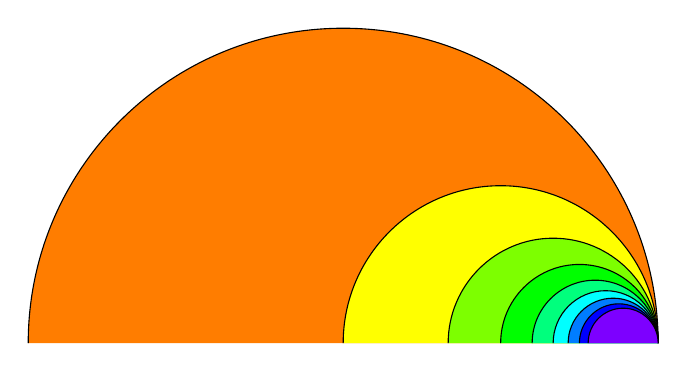
\begin{tikzpicture}% TikzPython id = (0) 
	\draw[fill={rgb,255:red, 255; green, 125; blue, 0 }] (0, 0) arc (0:180:4.0cm);
	\draw[fill={rgb,255:red, 255; green, 255; blue, 0 }] (0, 0) arc (0:180:2.0cm);
	\draw[fill={rgb,255:red, 125; green, 255; blue, 0 }] (0, 0) arc (0:180:1.3333333333333333cm);
	\draw[fill={rgb,255:red, 0; green, 255; blue, 0 }] (0, 0) arc (0:180:1.0cm);
	\draw[fill={rgb,255:red, 0; green, 255; blue, 125 }] (0, 0) arc (0:180:0.8cm);
	\draw[fill={rgb,255:red, 0; green, 255; blue, 255 }] (0, 0) arc (0:180:0.6666666666666666cm);
	\draw[fill={rgb,255:red, 0; green, 125; blue, 255 }] (0, 0) arc (0:180:0.5714285714285714cm);
	\draw[fill={rgb,255:red, 0; green, 0; blue, 255 }] (0, 0) arc (0:180:0.5cm);
	\draw[fill={rgb,255:red, 125; green, 0; blue, 255 }] (0, 0) arc (0:180:0.4444444444444444cm);
\end{tikzpicture}
\end{center}
\end{center}
\end{center}
\end{center}
\end{center}
\end{center}
\end{center}
\end{center}
\end{center}
\end{center}
\end{center}
\end{center}
\end{center}
\end{center}
\end{center}
\end{center}
\end{center}
\end{center}
\end{center}
